%%%%%%%%%%%%%%%%%%%%%%%%%%%%%%%%%%%%%%%%%
% Beamer Presentation
% LaTeX Template
% Version 1.0 (10/11/12)
%
% This template has been downloaded from:
% http://www.LaTeXTemplates.com
%
% License:
% CC BY-NC-SA 3.0 (http://creativecommons.org/licenses/by-nc-sa/3.0/)
%
%%%%%%%%%%%%%%%%%%%%%%%%%%%%%%%%%%%%%%%%%

%----------------------------------------------------------------------------------------
%	PACKAGES AND THEMES
%----------------------------------------------------------------------------------------

\documentclass{beamer}

\mode<presentation> {

% The Beamer class comes with a number of default slide themes
% which change the colors and layouts of slides. Below this is a list
% of all the themes, uncomment each in turn to see what they look like.

%\usetheme{default}
%\usetheme{AnnArbor}
%\usetheme{Antibes}
%\usetheme{Bergen}
%\usetheme{Berkeley}
%\usetheme{Berlin}
%\usetheme{Boadilla}
%\usetheme{CambridgeUS}
%\usetheme{Copenhagen}
%\usetheme{Darmstadt}
%\usetheme{Dresden}
%\usetheme{Frankfurt}
%\usetheme{Goettingen}
%\usetheme{Hannover}
%\usetheme{Ilmenau}
%\usetheme{JuanLesPins}
%\usetheme{Luebeck}
\usetheme{Madrid}
%\usetheme{Malmoe}
%\usetheme{Marburg}
%\usetheme{Montpellier}
%\usetheme{PaloAlto}
%\usetheme{Pittsburgh}
%\usetheme{Rochester}
%\usetheme{Singapore}
%\usetheme{Szeged}
%\usetheme{Warsaw}

% As well as themes, the Beamer class has a number of color themes
% for any slide theme. Uncomment each of these in turn to see how it
% changes the colors of your current slide theme.

%\usecolortheme{albatross}
%\usecolortheme{beaver}
%\usecolortheme{beetle}
%\usecolortheme{crane}
%\usecolortheme{dolphin}
%\usecolortheme{dove}
%\usecolortheme{fly}
%\usecolortheme{lily}
%\usecolortheme{orchid}
%\usecolortheme{rose}
%\usecolortheme{seagull}
\usecolortheme{seahorse}
%\usecolortheme{whale}
%\usecolortheme{wolverine}

%\setbeamertemplate{footline} % To remove the footer line in all slides uncomment this line
%\setbeamertemplate{footline}[page number] % To replace the footer line in all slides with a simple slide count uncomment this line

%\setbeamertemplate{navigation symbols}{} % To remove the navigation symbols from the bottom of all slides uncomment this line
\setbeamertemplate{blocks}[rounded][shadow=false]
\setbeamertemplate{section in toc}{\inserttocsectionnumber.~\inserttocsection}


}

\usepackage{graphicx} % Allows including images
\usepackage{booktabs} % Allows the use of \toprule, \midrule and \bottomrule in tables


\usepackage{xcolor}
\usepackage{listings}

\definecolor{mGreen}{rgb}{0,0.5,0}
\definecolor{mGray}{rgb}{0.5,0.5,0.5}
\definecolor{mPurple}{rgb}{0.58,0,0.82}
\definecolor{backgroundColour}{rgb}{0.95,0.95,0.92}


\lstloadlanguages{{C}}

\lstdefinestyle{CStyle}{
   % backgroundcolor=\color{backgroundColour},   
    commentstyle=\color{mGreen},
    keywordstyle=\color{magenta},
    numberstyle=\tiny\color{mGray},
    stringstyle=\color{mPurple},
    basicstyle=\footnotesize,
    breakatwhitespace=false,         
    breaklines=true,                 
    captionpos=b,                    
    keepspaces=true,                 
    numbers=left,                    
    numbersep=5pt,                  
    showspaces=false,                
    showstringspaces=false,
    showtabs=false,                  
    tabsize=2,
    language=C,
    aboveskip=\smallskipamount,
    belowskip=\smallskipamount,
    mathescape=true,
    morekeywords = {assert},
    moredelim=**[is][\only<+>{\color{black}\lstset{style=highlight}}]{~}{~},
    literate= {|->}{{$\mapsto$}}1 {_L}{{$_L$}}1,
}

\lstdefinestyle{CStyleNoNum}{
   % backgroundcolor=\color{backgroundColour},   
    commentstyle=\color{mGreen},
    keywordstyle=\color{magenta},
    numberstyle=\tiny\color{mGray},
    stringstyle=\color{mPurple},
    basicstyle=\footnotesize,
    breakatwhitespace=false,         
    breaklines=true,                 
    captionpos=b,                    
    keepspaces=true,                 
    %numbers=left,                    
    %numbersep=5pt,                  
    showspaces=false,                
    showstringspaces=false,
    showtabs=false,                  
    tabsize=2,
    language=C,
    aboveskip=\smallskipamount,
    belowskip=\smallskipamount,
    mathescape=true,  
    morekeywords = {assert},
    moredelim=**[is][\only<+>{\color{black}\lstset{style=highlight}}]{~}{~},
    literate= {|->}{{$\mapsto$}}1 {_L}{{$_L$}}1,
}

\lstdefinestyle{highlight}{
  keywordstyle=\color{magenta},
  commentstyle=\color{mGreen},
}

\lstdefinestyle{CStyleOverlay}{
   % backgroundcolor=\color{backgroundColour}, 
    %basicstyle=\footnotesize,    
    basicstyle=\footnotesize\color{black!40},
  	keywordstyle=\color{black!40},%{red!40},
  	commentstyle=\color{black!40},%{green!40},  
    %commentstyle=\color{mGreen},
    %keywordstyle=\color{magenta},
    numberstyle=\tiny\color{mGray},
    stringstyle=\color{mPurple},
    breakatwhitespace=false,         
    breaklines=true,                 
    captionpos=b,                    
    keepspaces=true,                 
    numbers=left,                    
    numbersep=5pt,                  
    showspaces=false,                
    showstringspaces=false,
    showtabs=false,                  
    tabsize=2,
    language=C,
    aboveskip=\smallskipamount,
    belowskip=\smallskipamount,
    mathescape=true,
    morekeywords = {assert},
    moredelim=**[is][\only<+-+(1)>{\color{black}\lstset{style=highlight}}]{~}{~},
    moredelim=**[is][\only<.(1)>{\color{black}\lstset{style=highlight}}]{@@}{@@},
    moredelim=**[is][\only<6>{\color{black}\lstset{style=highlight}}]{£}{£},
    moredelim=**[is][\only<6>{\color{black}\lstset{style=highlight}}]{**}{**},
    literate= {|->}{{$\mapsto$}}1 {_L}{{$_L$}}1 {_(L-1)}{{$_{L-1}$}}3,
    escapeinside={µ}{µ},
    %moredelim=**[is][\only<+>{\color{red}}]{@@}{@@},
}
\let\origthelstnumber\thelstnumber
\makeatletter
\newcommand*\Suppressnumber{%
  \lst@AddToHook{OnNewLine}{%
    \let\thelstnumber\relax%
     \advance\c@lstnumber-\@ne\relax%
    }%
}
\newcommand*\Reactivatenumber[1]{%
  \setcounter{lstnumber}{\numexpr#1-1\relax}
  \lst@AddToHook{OnNewLine}{%
   \let\thelstnumber\origthelstnumber%
   \refstepcounter{lstnumber}
  }%
}

\makeatother
\usepackage{tikz}


\usepackage{amsmath}
\usepackage{amssymb}
\usepackage[inference]{semantic}
\usepackage{xargs}
\usepackage{etoolbox}

\makeatletter
\def\@myenvname{equation}
\newcommand{\eqIfNoEq}[1]{%
  \ifx\@currenvir\@myenvname
    #1
  \else
    \begin{equation}#1
    \end{equation}
  \fi}
\newcommand{\eqIfNoMM}[1]{%
  \ifmmode
    #1
  \else
    \begin{equation}#1
    \end{equation}
  \fi}
\makeatother

\let\oldinference\inference
%\renewcommand{\inference}[2]{\[\oldinference{#1}{#2}\]}
\renewcommandx*\inference[3][3]{
\ifstrempty{#3}{
\eqIfNoEq{\oldinference{#1}{#2}}
}{
\eqIfNoEq{\oldinference{#1}{#2\tagsc{#3}}}
}
}

\newbool{shouldUseCompile}
\setbool{shouldUseCompile}{true}
\newcommandx*\triple[7][2,3,6,7]{\{#1\}^{#2}_{#3}\ #4\ \{#5\}^{#6}_{#7}} %\ifmmode to enforce math mode, but this should work without the checks
\newcommandx*\compile[3][3]{\ifbool{shouldUseCompile}{#1 \leadsto_{#3} #2}{#1}}

\usepackage{enumitem}
\setitemize{label=\usebeamerfont*{itemize item}%
  \usebeamercolor[fg]{itemize item}
  \usebeamertemplate{itemize item}}

\newcommandx*\simrelcom[2]{
{#1} \ R\ {#2}
}
\newcommandx*\backtranslation[1]{\langle\langle #1 \rangle\rangle}



%blue boxes
\definecolor{myblue}{rgb}{.84, .84, .95}
\usepackage{empheq}
\setbeamercolor{block body}{bg=myblue}


\newlength\mytemplen
\newsavebox\mytempbox

\makeatletter
\newcommand\mybluebox{%
    \@ifnextchar[%]
       {\@mybluebox}%
       {\@mybluebox[0pt]}}

\def\@mybluebox[#1]{%
    \@ifnextchar[%]
       {\@@mybluebox[#1]}%
       {\@@mybluebox[#1][0pt]}}

\def\@@mybluebox[#1][#2]#3{
    \sbox\mytempbox{#3}%
    \mytemplen\ht\mytempbox
    \advance\mytemplen #1\relax
    \ht\mytempbox\mytemplen
    \mytemplen\dp\mytempbox
    \advance\mytemplen #2\relax
    \dp\mytempbox\mytemplen
    \colorbox{myblue}{\hspace{1em}\usebox{\mytempbox}\hspace{1em}}}

\makeatother

%gets rid of footer
%will override 'frame number' instruction above
%comment out to revert to previous/default definitions
\setbeamertemplate{footline}{}
%gets rid of bottom navigation symbols
\setbeamertemplate{navigation symbols}{}

%Gannt chart stuff:
\usepackage{pgfgantt}
\usepackage{xparse}
\usepackage{enumitem}% http://ctan.org/pkg/enumitem

\NewDocumentCommand\textganttbar{O{} O{} mmmm}{%
    \ganttbar[#1,bar/.append style={alias=tmp}]{#3}{#5}{#6}
    \node [font=\footnotesize,at={(tmp)},#2]  {#4};
}

\tikzset{
  above bar/.style={
    at={(tmp.north)},anchor=south
    },
  below bar/.style={
    at={(tmp.south)},anchor=north
    }
}

%Rotated Tabular labels
\usepackage{array,multirow}
\newcolumntype{M}[1]{>{\centering\arraybackslash}m{#1}}
\usepackage{colortbl}% http://ctan.org/pkg/xcolor

\newcommand{\blacksubs}[1]{_{\color{black}\text{#1}}}
\newcommand{\blacksupers}[1]{^{\color{black}\text{#1}}}

\usepackage{stmaryrd}
\newcommand{\compsymb}[1]{\llbracket #1 \rrbracket}

%----------------------------------------------------------------------------------------
%	TITLE PAGE
%----------------------------------------------------------------------------------------

\title[Linear Capability Verification]{Linear capabilities for fully abstract
compilation of separation-logic-verified code} % The short title appears at the bottom of every slide, the full title is only on the title page

\author[Thomas Van Strydonck]{\underline{Thomas Van Strydonck} \and Dominique Devriese \and Frank Piessens} % Your name
\institute[KU Leuven] % Your institution as it will appear on the bottom of every slide, may be shorthand to save space
{
KU Leuven \\ % Your institution for the title page
\medskip
\textit{thomas.vanstrydonck@cs.kuleuven.be} % Your email address
}
\date{\today} % Date, can be changed to a custom date

\begin{document}

%Showing off the current section
\AtBeginSection[]{
  \begin{frame}{Outline}
  \small \tableofcontents[currentsection, hideothersubsections]
  \end{frame} 
}

%%Start of the presentation

\begin{frame}
\titlepage % Print the title page as the first slide 
\end{frame}



\begin{frame}[plain,c]
%\frametitle{A first slide}
\begin{center}
\Huge Linear capabilities for\\  \textbf{\underline{fully abstract}}
compilation of separation-logic-verified code
\end{center}
\end{frame}


\begin{frame}
\frametitle{Overview} % Table of contents slide, comment this block out to remove it
\tableofcontents % Throughout your presentation, if you choose to use \section{} and \subsection{} commands, these will automatically be printed on this slide as an overview of your presentation
\end{frame}

%------------------------------------------------

\section{Full abstraction}

\begin{frame}
\frametitle{Full abstraction (FA)} %Mention secure compilation?
 %\setbeamercovered{transparent}
\begin{block}{Intuition}<1->
Attacking the compiled code is as hard as attacking the source code \\[1em]%Even though the target language is usually lower level and hence more powerful as an attacker
%Fully abstract compiler $\Rightarrow$ compiled code upholds contracts\\
\end{block}
\only<2-3>{
\begin{block}{Definition of FA} %Q? or is this too trivial? It was a confusing bit for me at the start
= reflection and preservation of contextual equivalence $\simeq_{ctx}$ \\
\vspace{-1em}
\begin{align*}&s\simeq_{ctx}s' \Leftrightarrow \compsymb{s}\simeq_{ctx}\compsymb{s'}\\
&\text{where } x\simeq_{ctx}x'\equiv \forall C: C[x]\Downarrow\ \Leftrightarrow C[x']\Downarrow
\end{align*}
$\supseteq$ preservation of integrity and confidentiality properties \\
\end{block}
} 
\only<3>{
\textbf{Methodology}:
Change the source language by $\compsymb{\cdot}$ + prove FA\\
\quad $\Rightarrow$ Change does not alter security aspects\\
\quad eg. CFI, notion of private fields, \ldots  
}
 %idea: we take contextual equivalence to mean our (sensible) notion of program equivalence, and say that programs are equivalent in the source iff. they are equivalent in the source. In other words, they don't behave differently in target vs source
 %useful when interacting with code at a lower level of abstraction
 %eg. prove preservation of control flow, private fields stay private
 %template: compile language away, prove that FA holds -> (OR: denotational semantics) 
\end{frame}

%------------------------------------------------
\section{Our application of full abstraction}

\begin{frame}
\frametitle{Problem: Preserving verification during compilation}

\begin{columns}
\begin{column}{0.65\textwidth}
\begin{itemize}
\item Separation logic in verification tools
	\begin{itemize}
	\item Sound
	\item Modular
	\end{itemize}
\item \textbf{Problem}: Guarantees \emph{lost} in untrusted context %why? keeping references etc; multithreading,...
\item \textbf{Solution}: Fully abstract compiler enforces separation logic contracts  %compiles vf -> uvf
\item Fully abstract compiler $\Rightarrow$ compiled code upholds contracts
\end{itemize}
\end{column}
\begin{column}{0.37\textwidth}
\def\firstcircle{(0,0) circle (2cm)}
\def\secondcircle{(0,0) circle (1.3cm)}
\colorlet{circle edge}{black!100}
\colorlet{circle area}{black!0}
\tikzset{filled/.style={fill=circle area, draw=circle edge, thick}, outline/.style={draw=circle edge, thick}}

%\setlength{\parskip}{5mm}
\begin{tikzpicture}
    \draw[outline] \firstcircle node {Verified Cmpnt};
    \draw[outline] \secondcircle node {};
    \node at (0,-1.6) (nodeA) {Context};
\end{tikzpicture}
\end{column}
\end{columns}
\end{frame}



\begin{frame}[plain,c]
%\frametitle{A first slide}

\begin{center}
\Huge Linear capabilities for\\  fully abstract
compilation of \textbf{\underline{separation-logic-verified}} code
\end{center}
\end{frame}


\begin{frame}[fragile]
\frametitle{Separation Logic} 
\begin{itemize}
\item Substructural logic (linear aspects)
\item Program verification
\begin{itemize}
\item Sound %proof implies correct
\item Modular %per-module proofs
\end{itemize}
\item Contract-based, eg. :\\
\begin{columns}%<0>
\begin{column}{0.55\textwidth}
\begin{lstlisting}[style=CStylenoNum, captionpos = t, xleftmargin = 4em]
void p(int x,int *data)
//@pre data |-> _ * x > 0;
//@post data |-> x;
{*data = x}
\end{lstlisting}
\end{column}
\begin{column}{0.45\textwidth}
Notation:
\begin{itemize}
\item $\textcolor{mGreen}{\ast}$, $\textcolor{mGreen}{\mapsto}$ (resource: permission)
\item @pre/post: contract\\
	\quad Consume/produce
\item Array resource notation:\\
	 \quad $\mapsto$[$a_1,\ldots, a_n$]
\end{itemize}
\end{column}
\end{columns}
\vspace{1em}
\item Hoare-logic-style program proofs: $\Rightarrow \triple{P}{c}{Q}$\\
	\quad Functions: $\triple{@pre}{BODY}{@post}$
\end{itemize}
\end{frame}

%------------------------------------------------

\begin{frame}[fragile]
\frametitle{Motivating example}
\begin{figure}[ht]
\begin{tabular}{c|M{.4\textwidth}|M{.4\textwidth}}
& \textbf{Verified Component}  & \textbf{Context Declaration} \\
\hline%\\[-1.20em]
\rotatebox[origin=c]{90}{\textbf{Source}}&
{\begin{lstlisting}[style=CStyle,numbers=none,belowskip=-1em]
void f(int* a)
//@pre n: a |-> [0]  
//@post n : a |-> [1]
{
	id(a); 
	a[0]=1;
}
\end{lstlisting}}
&
{\begin{lstlisting}[style=CStyle,numbers=none,belowskip=-1em]
void id(int* a)
//@pre n: a |-> [0]  
//@post n : a |-> [0]
\end{lstlisting}}\\
\end{tabular} 
%\caption{Motivating example: a verified component is interacting with an untrusted context}
\label{trivialexample}
%\vspace*{-10pt}
\end{figure} %NOTE; we name resources for reasons of compilation
\begin{itemize}
\item SOA: compilers erase contracts
\item Untrusted function $id$ can:
	\begin{itemize}
	\item Overread/-write using $a$, copy $a$
	\item Not satisfy postcondition (eg. $a[0] =2$)
	\end{itemize}
\item \textbf{NOT fully abstract!} %Because contracts are not upheld!
\end{itemize}
\end{frame}

%------------------------------------------------

\begin{frame}
\frametitle{The compiler}
\begin{columns}
\begin{column}{0.45\textwidth}
	\begin{block}{Source language}
	\begin{itemize}
	\item Regular verified C code
	\item \emph{Separation logic} annotated
		%\begin{itemize}
		%\item e.g. VeriFast syntax for concreteness
		%\end{itemize}
	\end{itemize}
	\end{block}
\end{column}
\begin{column}{0.08\textwidth}
	\begin{figure}
	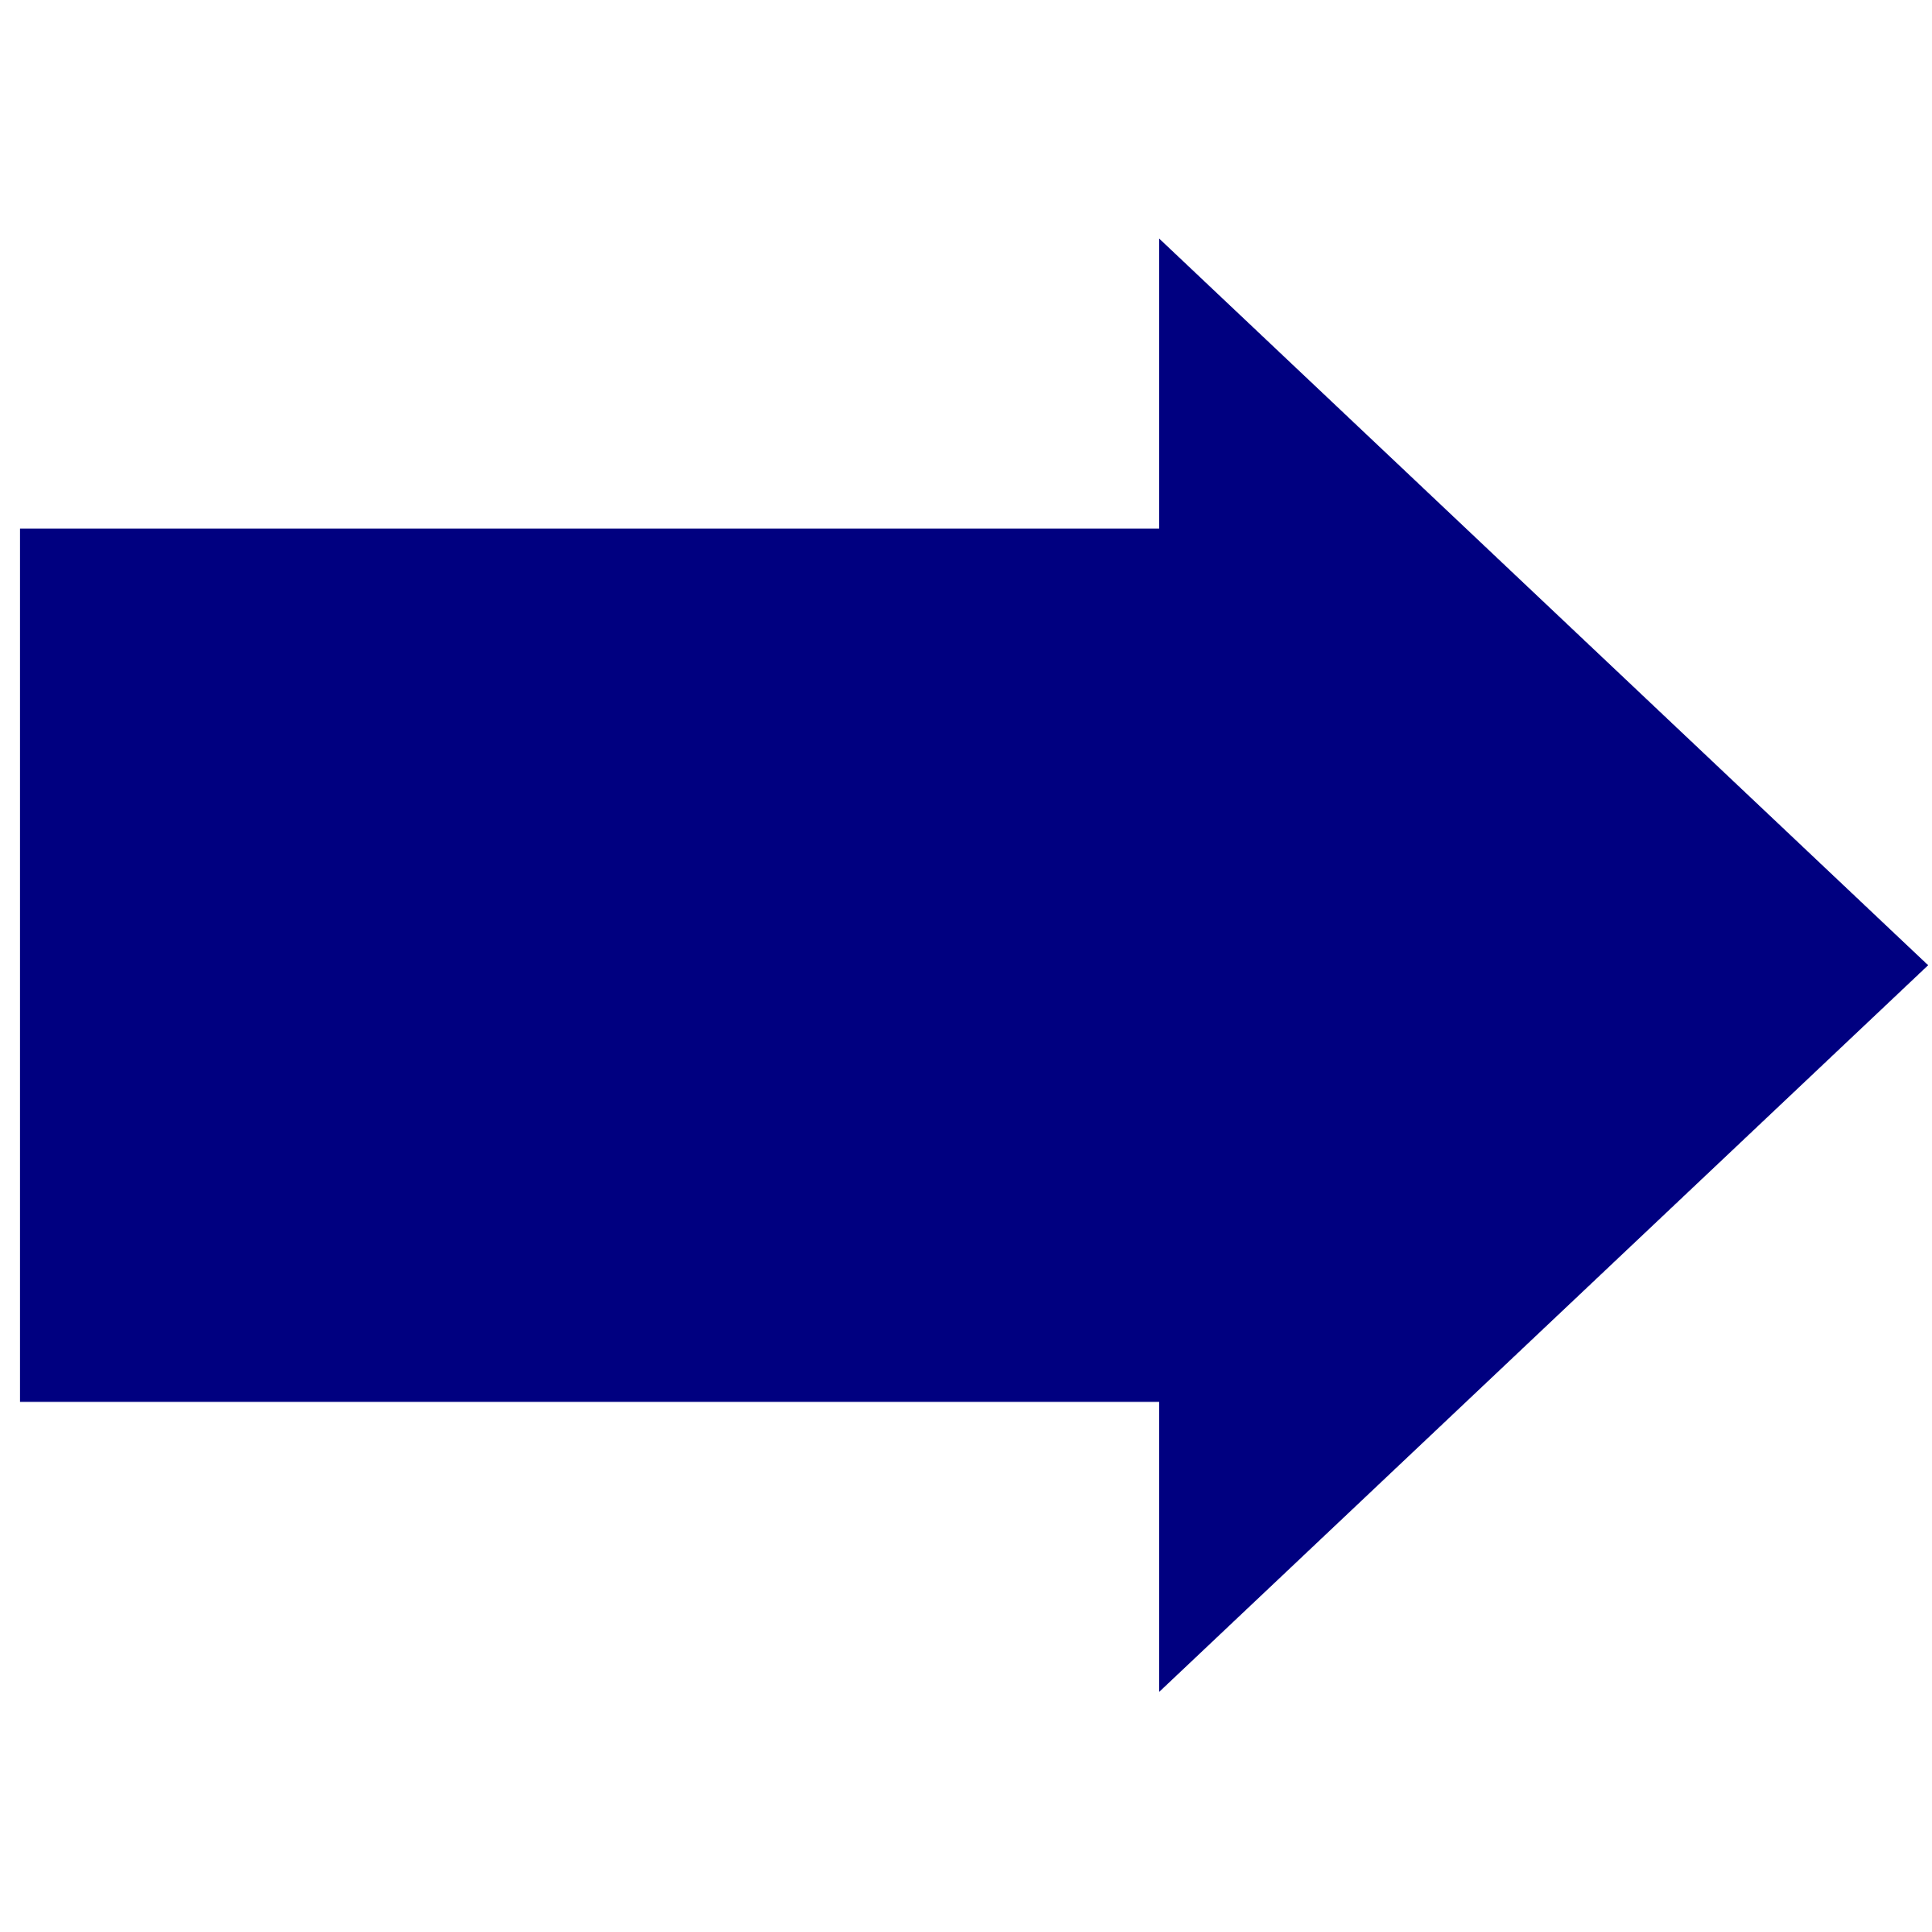
\includegraphics[width=0.8\linewidth]{BlueArrow}
	\end{figure}
\end{column}
\begin{column}{0.45\textwidth}
    \begin{block}{Target language}
	\begin{itemize}
	\item Regular unverified C code
	\item \textbf{Language enhancement to allow full abstraction???} \\
	\end{itemize}
	\end{block}
\end{column}
\end{columns}
%\vspace{1em}
\center No assembly hassle in C, but still unsafe (powerful attacker).

 %compiles vf -> uvf
\end{frame}

\begin{frame}[fragile]
\frametitle{What (language) enhancements do we need?}
\begin{figure}[ht]
\begin{tabular}{c|M{.4\textwidth}|M{.4\textwidth}}
& \textbf{Verified Component}  & \textbf{Context Declaration} \\
\hline%\\[-1.20em]
\rotatebox[origin=c]{90}{\textbf{Source}}&
{\begin{lstlisting}[style=CStyle,numbers=none,belowskip=-1em]
void f(int* a)
//@pre n: a |-> [0]  
//@post n : a |-> [1]
{
	id(a); 
	a[0]=1;
}
\end{lstlisting}}
&
{\begin{lstlisting}[style=CStyle,numbers=none,belowskip=-1em]
void id(int* a)
//@pre n: a |-> [0]  
//@post n : a |-> [0]
\end{lstlisting}}\\
\end{tabular} 
%\caption{Motivating example: a verified component is interacting with an untrusted context}
\label{trivialexample}
%\vspace*{-10pt}
\end{figure} %NOTE; we name resources for reasons of compilation
Recall, $id$ can:
	\begin{itemize}
	\item Overread/-write using $a$, copy $a$\\
	\quad $\Rightarrow$ \textbf{Capabilities} implement POLA\\
	\quad $\Rightarrow$ \textbf{Linear Capabilities} prevent copying
	\item Not satisfy postcondition (eg. $a[0] =2$)\\
	\quad $\Rightarrow$ \textbf{Checking functions aka. stubs}
	\end{itemize}
\end{frame}

\begin{frame}[plain,c]
%\frametitle{A first slide}

\begin{center}
\Huge \underline{\textbf{Linear capabilities}} for\\  fully abstract
compilation of separation-logic-verified code
\end{center}

\end{frame}


%------------------------------------------------

\begin{frame}
\frametitle{(Linear) Capabilities}

\begin{columns}
\begin{column}{0.5\textwidth}
	\textbf{Capability}: %Q? leave this out/reduce to one line? Or add figure? + source for figure?
\begin{itemize}
\item Unforgeable memory pointer
\item Grants permissions on memory region
\item Fine-grained memory protection
\item Capability machines (ex CHERI)
\end{itemize}
\end{column}
\begin{column}{0.5\textwidth}
\begin{figure}
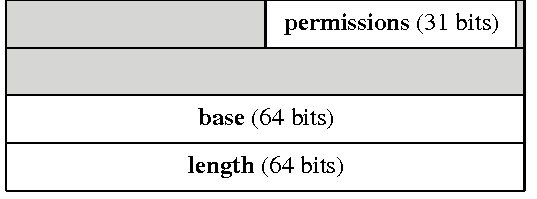
\includegraphics[width=\linewidth]{Capability}%Q? Reference? https://www.semanticscholar.org/paper/The-CHERI-capability-model-Revisiting-RISC-in-an-a-Woodruff-Watson/0657eb7e069c2c2c7cae6636704e0f7fb3bcd9fc
\end{figure}
\end{column}
\end{columns}
\vspace{.5em}

 %compiles vf -> uvf
%\textbf{Sealed Capability}: %Q? Delete
%Unaccessible until unsealed using an appropriate seal.
%\vspace{.5em}

\textbf{Linear Capability}: %Fits very well with consuming and producing in separation logic = linear aspects of separation logic
\begin{itemize}
\item Linearity = one-use! cfr e.g. Linear Logic
\item Non-copyable
$\Rightarrow$ callers/callees cannot keep copies
\item Intuitive: separation logic is linear
\end{itemize}
\end{frame}


%------------------------------------------------


\begin{frame}
\frametitle{Goal: proving that contracts are compiled away safely by proving full abstraction}
 %\setbeamercovered{transparent}
\begin{columns}%<0>
\begin{column}{0.45\textwidth}
	\begin{block}{Source language}
	\begin{itemize}
	\item Regular verified C code
	\item \emph{Separation logic} annotated
		\begin{itemize}
		\item e.g. VeriFast syntax for concreteness
		\end{itemize}
	\end{itemize}
	\end{block}
\end{column}
\begin{column}{0.08\textwidth}
	\begin{figure}
	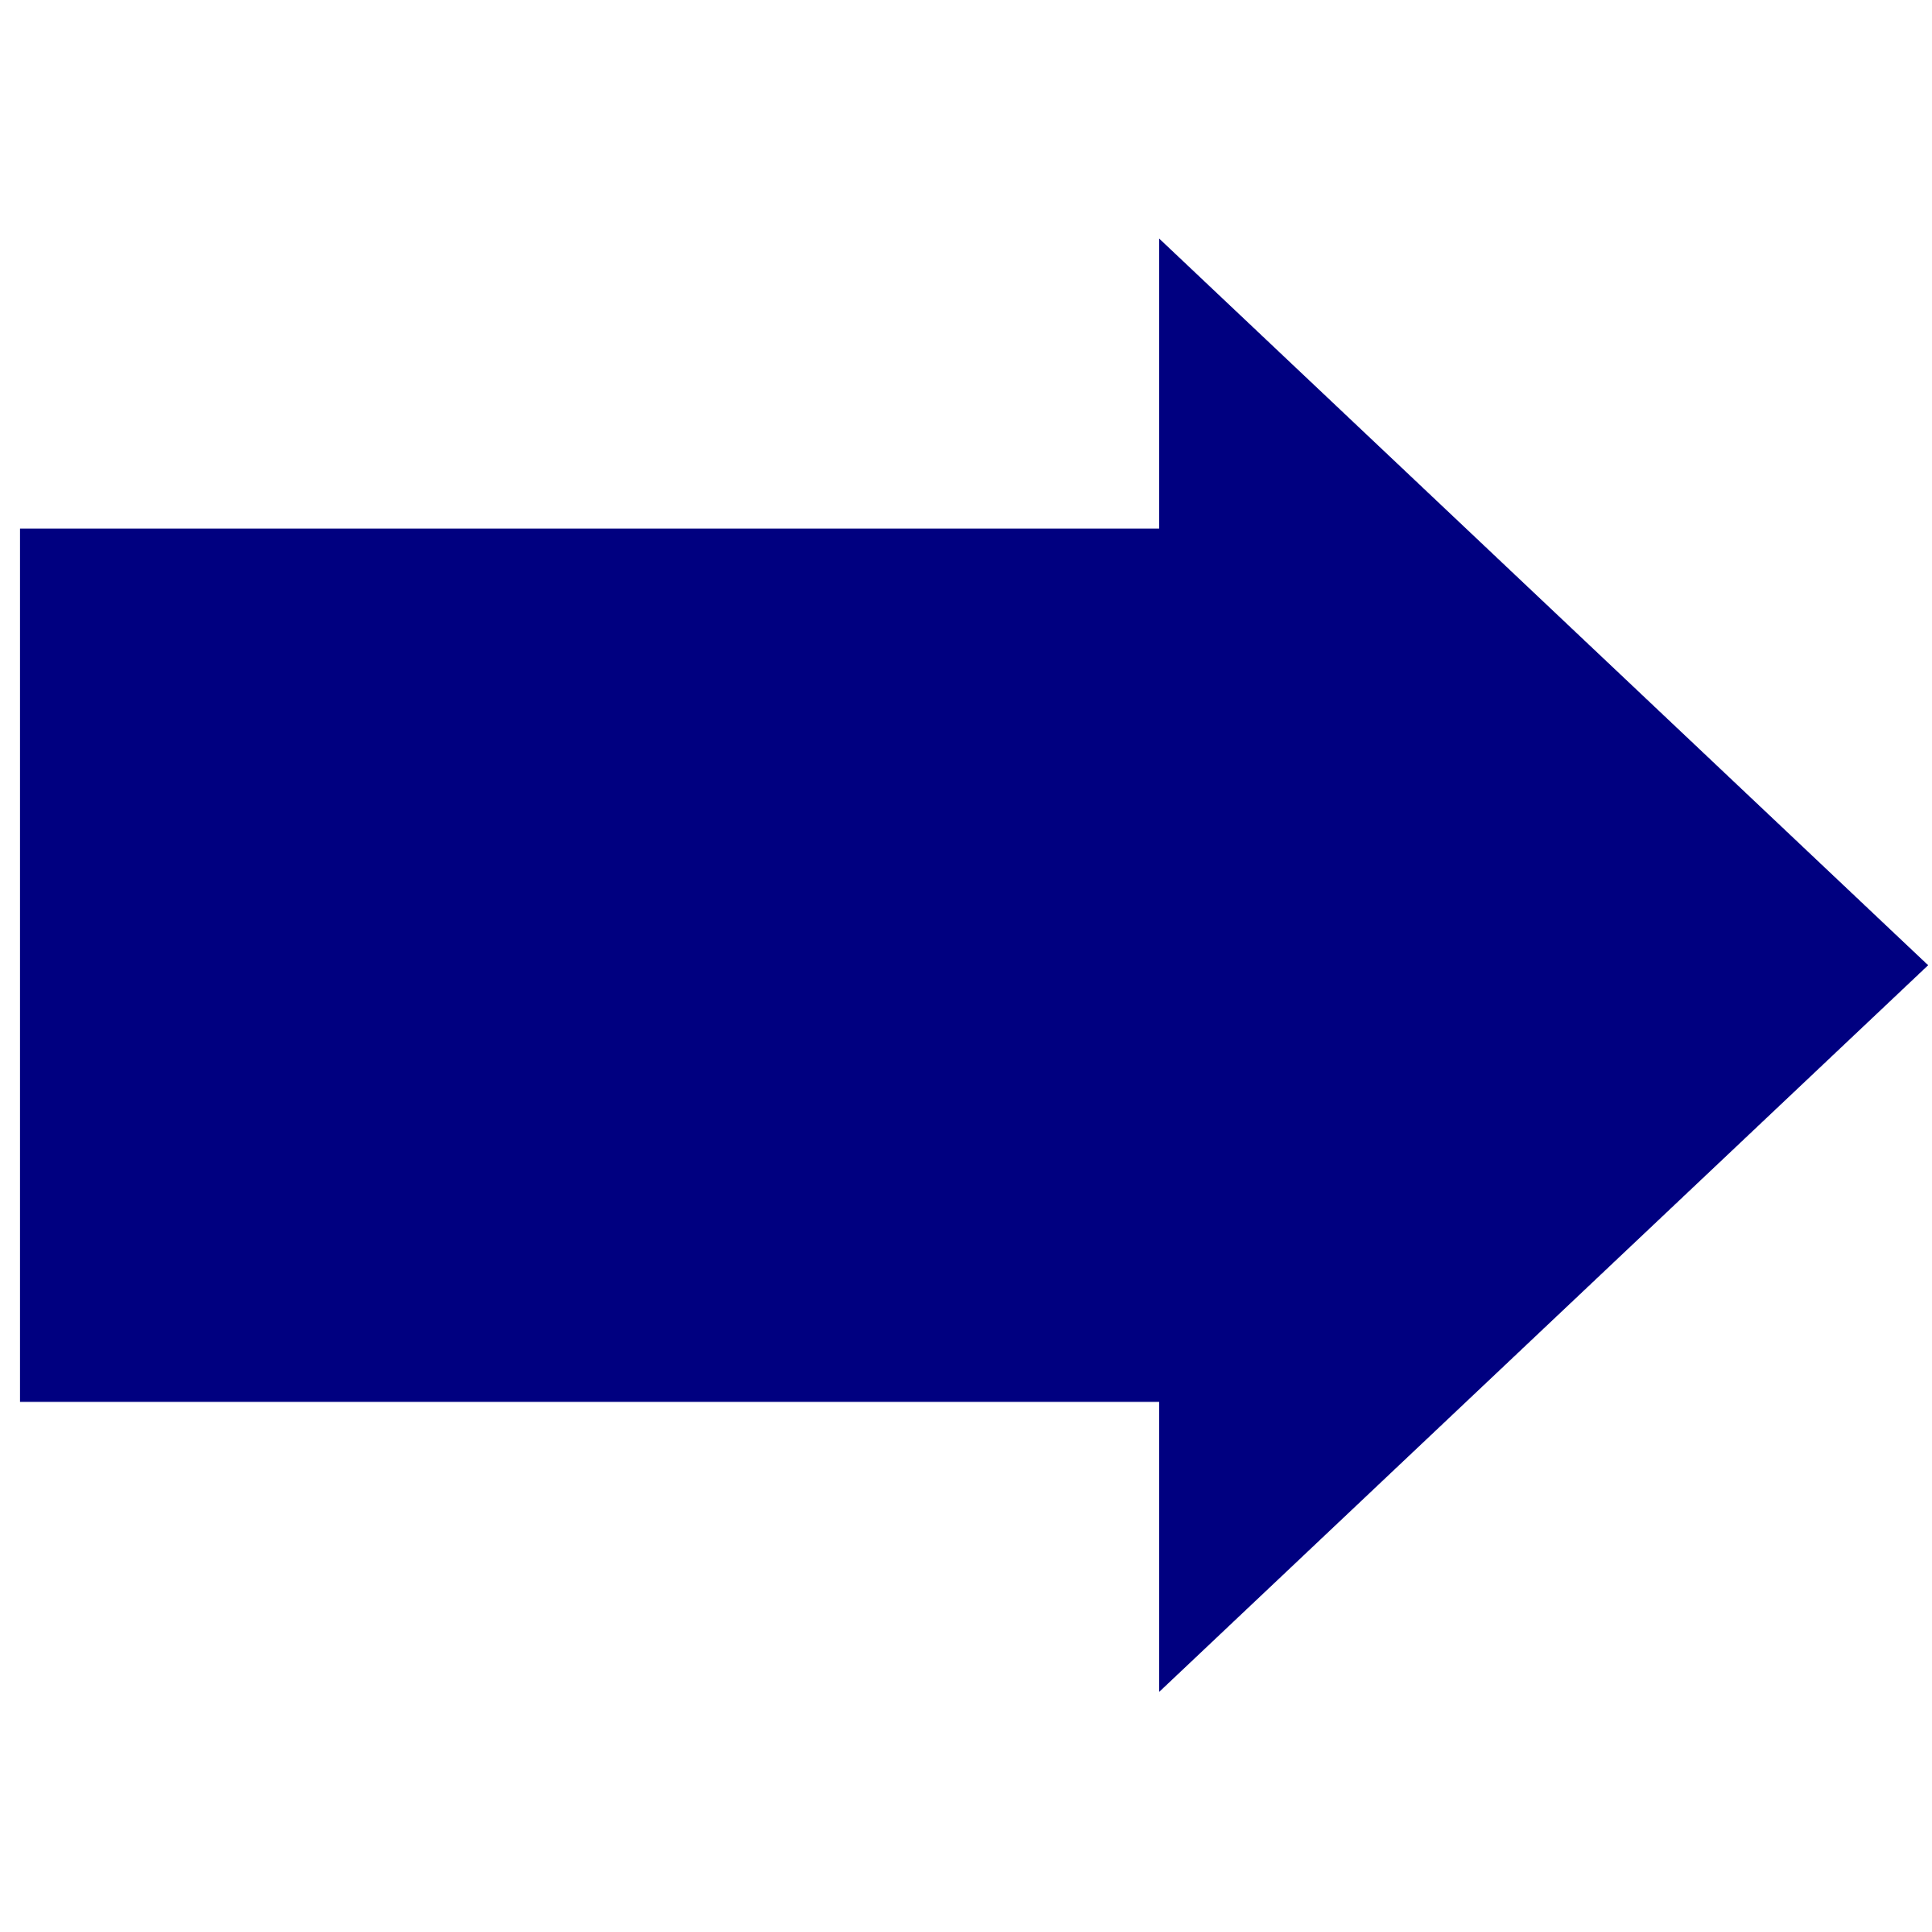
\includegraphics[width=0.8\linewidth]{BlueArrow}
	\end{figure}\vspace{-2em}
	\center \textbf{FA!}
\end{column}
\begin{column}{0.45\textwidth}
    \begin{block}{Target language}
	\begin{itemize}
	\item Regular unverified C code
	\item Support for \emph{capabilities}\\
		\begin{itemize}
		\item CHERI-inspired 
		\item Linear capabilities
		%\item Sealed capabilities %Q? Do we still need these? e.g. nested arrays wont contain nested capabilities; the nesting of capabilities was only a problem wiht AP's
		\end{itemize}
	\end{itemize}
	\end{block}
\end{column}
\end{columns}
\vspace{1em}
\centering
\textbf{Related work (Agten et al.)} %Q? maybe leave out? This is super relevant though, and underscores the advantage of fine-grainedness of capabilities wrt PMAs, but not everyone might know thi
\begin{itemize}
\item \centering
Different hardware primitives\\%PMA's instead of capabilities\\
	$\Rightarrow$ Less fine-grained
\item \centering
Integrity, \emph{not} confidentiality
\end{itemize}
\end{frame}

%------------------------------------------------
\section{Compilation by example}

%------------------------------------------------

\begin{frame}[fragile]
\frametitle{Compilation: Intuition}
\begin{columns}
\begin{column}{0.6\textwidth}
\begin{itemize}
\item Resources reified into linear capabilities
	\begin{itemize}
	\item Behave linearly
	\item Contain all permissions
	%\item Passed to/from functions
	\item This is why we \textbf{name} heap resources!
	\end{itemize}
\item Original pointers become addresses
	\begin{itemize}
	\item Regular ints\footnotemark
	\item Lose all permission
	\item Kept for address operations
	\end{itemize} 
%\item Enforcing function contracts for
%	\begin{itemize}
%	\item Incalls
%	\item Outcalls
%	\end{itemize}
%	$\Rightarrow$ Stubs
\end{itemize}

\end{column}

\begin{column}{0.4\textwidth}

\begin{center}
\begin{tabular}{c}
\begin{lstlisting}[style=CStyleNoNum, captionpos = t]
//{c1: n |-> [_]_L}
n: int*
\end{lstlisting}
\end{tabular}
\end{center}

\vspace{-.5em}
\begin{figure}[h]
\centering

\includegraphics[width=0.20\linewidth]{BlueArrowVertical}
\end{figure}
\vspace{-1em}

\begin{center}
\begin{tabular}{c}
\begin{lstlisting}[style=CStyleNoNum, captionpos = t]
c1: int* (linear)
 n: int
\end{lstlisting}
\end{tabular}
\end{center}

\end{column}
\end{columns}
\vspace{1em}

$\Rightarrow$ \emph{Separation-logic-proof-directed}:
\qquad \begin{itemize}
\item \textbf{proof of} input program used as input
\item operations happen on resources, eg. $a[0] \Rightarrow_{\compsymb{\cdot}} n[0]$
\end{itemize}
\footnotetext[1]{This is a slight simplification}
\end{frame}

%------------------------------------------------

\begin{frame}[fragile]
\frametitle{Motivating example: overread/overwrite/copy}
\begin{figure}[ht]
\begin{tabular}{c|M{.4\textwidth}|M{.4\textwidth}}
& \textbf{Verified Component}  & \textbf{Context Declaration} \\
\hline%\\[-1.20em]
\rotatebox[origin=c]{90}{\textbf{Source}}&
{\begin{lstlisting}[style=CStyle,numbers=none,belowskip=-1em]
void f(int* a)
//@pre n: a |-> [0]  
//@post n : a |-> [1]
{
	id(a); 
	a[0]=1;
}
\end{lstlisting}}
&
{\begin{lstlisting}[style=CStyle,numbers=none,belowskip=-1em]
void id(int* a)
//@pre n: a |-> [0]  
//@post n : a |-> [0]
\end{lstlisting}}\\


\hline


\rotatebox[origin=c]{90}{\textbf{Target}}&
{\begin{lstlisting}[style=CStyle,numbers=none,belowskip=-1em]
int* f(int a,int* n)
{
	n = id(a,n); 
	n[0]=1;
	return n;
}
\end{lstlisting}}&
{\begin{lstlisting}[style=CStyle,numbers=none,belowskip=-1em]
int* id(int a,int*n)
\end{lstlisting}}\\
\end{tabular} 
%\caption{Motivating example: a verified component is interacting with an untrusted context}
\label{trivialexample}
%\vspace*{-10pt}
\end{figure} %NOTE; we name resources for reasons of compilation

Prevented by: Linear capabilities + Proof-directed-compilation
\end{frame}

%------------------------------------------------

\begin{frame}[fragile]
\frametitle{Motivating example: postcondition}
\begin{figure}[ht]
\begin{tabular}{c|M{.42\textwidth}|M{.4\textwidth}}
& \textbf{Stub} & \textbf{Context Declaration} \\
\hline%\\[-1.20em]
\rotatebox[origin=c]{90}{\textbf{Source}}
&\cellcolor{gray!50!white!50}
&
{\begin{lstlisting}[style=CStyle,numbers=none,belowskip=-1em]
void id(int* a)
//@pre n: a |-> [0]  
//@post n : a |-> [0]
\end{lstlisting}}\\


\hline


\rotatebox[origin=c]{90}{\textbf{Target}}&
{\begin{lstlisting}[style=CStyle,numbers=none,belowskip=-1em]
int* id$\blacksubs{stub}$(int a,int* n)
{
	n = id(a,n); 
	assert(a == addr(n));
	assert(len(n) == 1);
	assert(n[0] == 0);
	return n;
}
\end{lstlisting}}&
{\begin{lstlisting}[style=CStyle,numbers=none,belowskip=-1em]
int* id(int a,int*n)
\end{lstlisting}}\\
\end{tabular} 
%\caption{Motivating example: a verified component is interacting with an untrusted context}
\label{trivialexample}
%\vspace*{-10pt}
\end{figure} %NOTE; we name resources for reasons of compilation

Prevented by: outcall stub
\end{frame}




%------------------------------------------------
\section{Conclusion and progress}

\begin{frame}
\frametitle{Conclusion}
\begin{itemize}
\item Compiler from verified C to unverified C with (linear) capabilities 
\item \textbf{Proven}: Full Abstraction\\
%\qquad$\Rightarrow$ Gave some proof intuition
%\item \textbf{State}: Pending POPL submission\\
\end{itemize}
\end{frame}

%------------------------------------------------
\section{Application to Rust }

\begin{frame}
\frametitle{Fully abstractly compiling Rust (IDEA STAGE)}

\begin{columns}
\begin{column}{0.65\textwidth}
\begin{itemize}
\item Ownership and borrowing; linear aspects
\quad $\Rightarrow$ Compile borrows to linear capabilities
\item Start from $\lambda_{Rust}$ in RustBelt
\end{itemize}
\end{column}
\begin{column}{0.37\textwidth}
\def\firstcircle{(0,0) circle (2cm)}
\def\secondcircle{(0,0) circle (1.3cm)}
\colorlet{circle edge}{black!100}
\colorlet{circle area}{black!0}
\tikzset{filled/.style={fill=circle area, draw=circle edge, thick}, outline/.style={draw=circle edge, thick}}

%\setlength{\parskip}{5mm}
\begin{tikzpicture}
    \draw[outline] \firstcircle node {
\includegraphics[width=.5\linewidth]{RustLogo}};
    \draw[outline] \secondcircle node {};
    \node at (0,-1.6) (nodeA) {Context};
\end{tikzpicture}
\end{column}
\end{columns}
\end{frame}

\end{document}
